\documentclass{beamer}
\usetheme{Antibes}
\usepackage{subcaption}
\usepackage{amsmath, amsfonts, amssymb}
\usepackage{physics}
\setbeamertemplate{footline}[frame number]
\setbeamersize{text margin left=5mm} 

\AtBeginSection[]{
  \begin{frame}
  \vfill
  \centering
  \begin{beamercolorbox}[sep=8pt,center,shadow=true,rounded=true]{title}
    \usebeamerfont{title}\insertsectionhead\par%
  \end{beamercolorbox}
  \vfill
  \end{frame}
}

\DeclareMathOperator*{\argmin}{arg\,min}

\title{Geometry of differential \textbf{geometry}: connections, flows, Lie brackets}
\author{Evgenii Samutichev}

\begin{document}

\maketitle

\begin{frame}{Outline}
    \small 
    \tableofcontents
\end{frame}

\section{Objects of study and how they look}
\begin{frame}{Warning: a little bit different notation}
    \begin{itemize}
        \item \textbf{Warning} Throughout this presentation I'll be using a different notation for the differential, namely 
        \begin{equation}
            \text{D}_x f[v] := \text{D}f(x)[v]
        \end{equation}
        \item I believe this makes equations more readable.
    \end{itemize}
\end{frame}
\subsection{Tensor fields}
\begin{frame}{Tensor fields}
    \begin{itemize}
        \item Scalar fields $f : \mathcal{M} \to \mathbb{R}$, living in $\mathfrak{F}(\mathcal{M})$, (0, 0)-tensor fields
        \item Vector fields $V : \mathcal{M} \to \text{T}\mathcal{M}$, living in $\mathfrak{X}(\mathcal{M})$, (1, 0)-tensor fields
        \item Covector fields $\alpha : \mathcal{M} \to \text{T}\mathcal{M}^*$, where $\alpha(x) \in (\text{T}_x\mathcal{M})^*$, (0, 1)-tensor fields. Example $x \to \text{D}_{x}f[\cdot]$ for $f \in \mathfrak{F}(\mathcal{M})$.
    \end{itemize}
    \begin{figure}[h!]
        \begin{subfigure}{.3333\textwidth}
            \centering  
            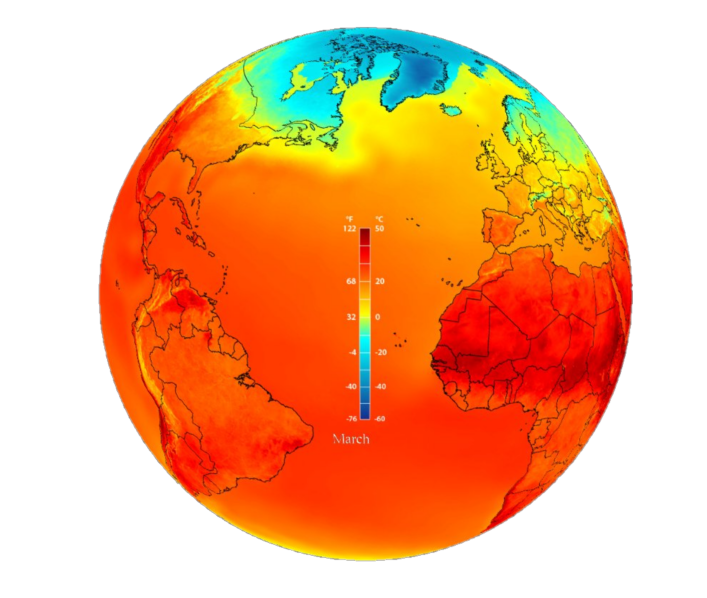
\includegraphics[width=0.9\textwidth]{images/temperature.png}
            \caption{A scalar field}
            \label{fig:sub1}
          \end{subfigure}%
          \begin{subfigure}{.3333\textwidth}
            \centering   
            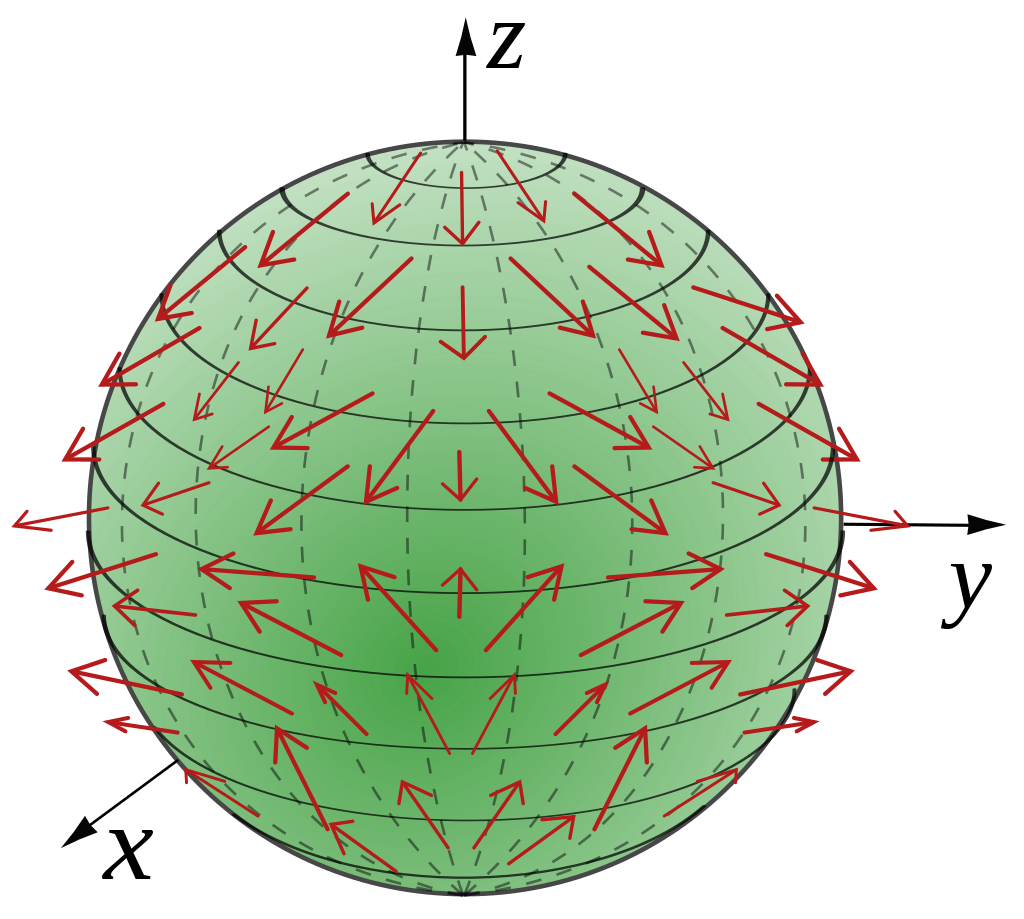
\includegraphics[width=0.9\textwidth]{images/vector_field_sphere.png}
            \caption{A vector field}
            \label{fig:sub2}
        \end{subfigure}%
        \begin{subfigure}{.3334\textwidth}
          \centering   
          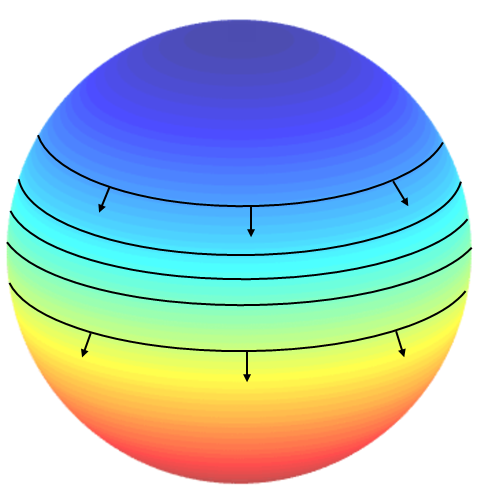
\includegraphics[width=0.8\textwidth]{images/covector field.png}
          \caption{A covector field}
          \label{fig:sub2}
      \end{subfigure}   
    \end{figure}
\end{frame}

\subsection{Riemannian metric}
\begin{frame}{Riemannian metric}
    \begin{itemize}
        \item \textbf{Riemannian metric} is a $(0, 2)$-tensor field, that is 
        \begin{equation}
            \langle \cdot, \cdot \rangle : \mathcal{M} \to T\mathcal{M}^* \times T\mathcal{M}^*, \text{ as } x \to \langle \cdot, \cdot \rangle_x 
        \end{equation}
        \item Judging by the signature, it "consumes" two vectors that are (1, 0)-tensors and returns a scalar. So $\langle V, W\rangle$ we defined on the last lecture is clearly a scalar field. 
        \item Why should we care? The chosen metric affects lengths of curves on the manifold as for $c : I \to \mathcal{M}$ its length is 
        \begin{equation}
            L(c) = \int_{I}{\sqrt{{\color{blue}\langle} c^\prime (t){\color{blue},} c^\prime(t){\color{blue}\rangle}_{{\color{blue}c(t)}}} dt}
        \end{equation}
        \item Thus, choosing the metric makes our rubber-sheet geometric structure of the manifold more rigid by fixing distances which are defined through the lengths of geodesic curves. 
    \end{itemize}
\end{frame}

\subsection{Previously defined operations}
\begin{frame}{Previously defined operations}
    \begin{itemize}
        \item Scalar field $f(x)$ to covector field $\text{D}_x f$
        \item Covector field $\text{D}_x f$ to vector field $\text{grad} f(x)$ as 
        \begin{equation}
              \text{D}_x f[u] = \langle \text{grad} f(x), u  \rangle_x
        \end{equation}
        \item \textbf{Definition 5.5 (3)} Two vector fields $V, W$ to scalar field $\langle V, W\rangle$ as 
        \begin{equation}
            \langle V, W\rangle(x) = \langle V(x), W(x)\rangle_x 
        \end{equation}
        \item Today we will discuss more of them. 
    \end{itemize}
\end{frame}

\section{Parallel transport problem}

\subsection{Change in vector fields on a plane}
\begin{frame}{Change in vector fields on a plane}
\begin{figure}[h!]
    \begin{subfigure}{.5\textwidth}
        \centering  
        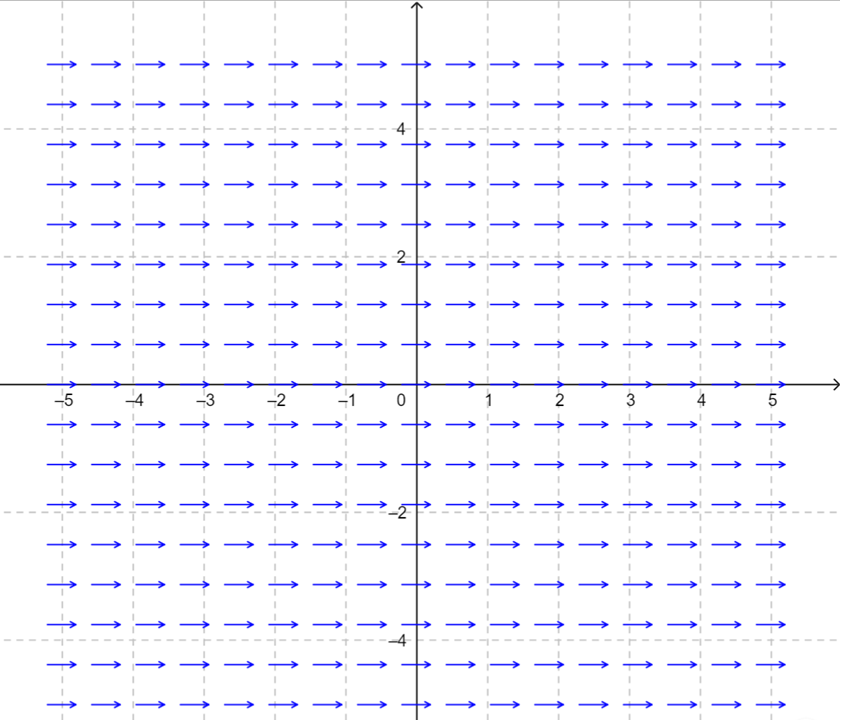
\includegraphics[width=0.9\textwidth]{images/vector_field_1.png}
        \caption{A constant vector field}
        \label{fig:sub1}
      \end{subfigure}%
      \begin{subfigure}{.5\textwidth}
        \centering   
        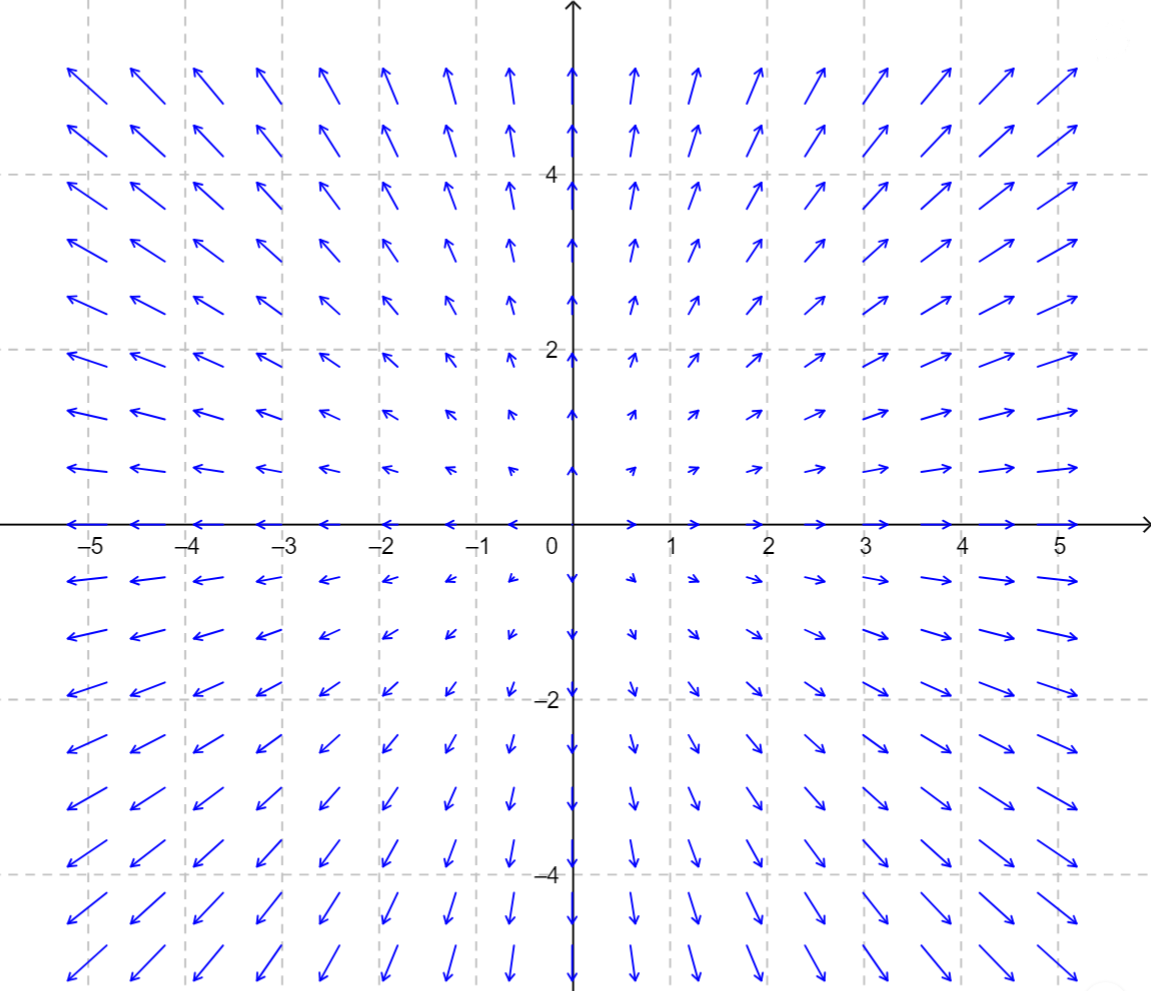
\includegraphics[width=0.9\textwidth]{images/vector_field_2.png}
        \caption{A non-constant vector field}
        \label{fig:sub2}
    \end{subfigure}  
\end{figure}
\begin{itemize}
    \item But what does it mean to be constant?
\end{itemize}
\end{frame}

\subsection{Parallel transport on the plane}
\begin{frame}{Parallel transport on the plane}
    \begin{figure}[h!]
        \begin{subfigure}{.5\textwidth}
            \centering  
            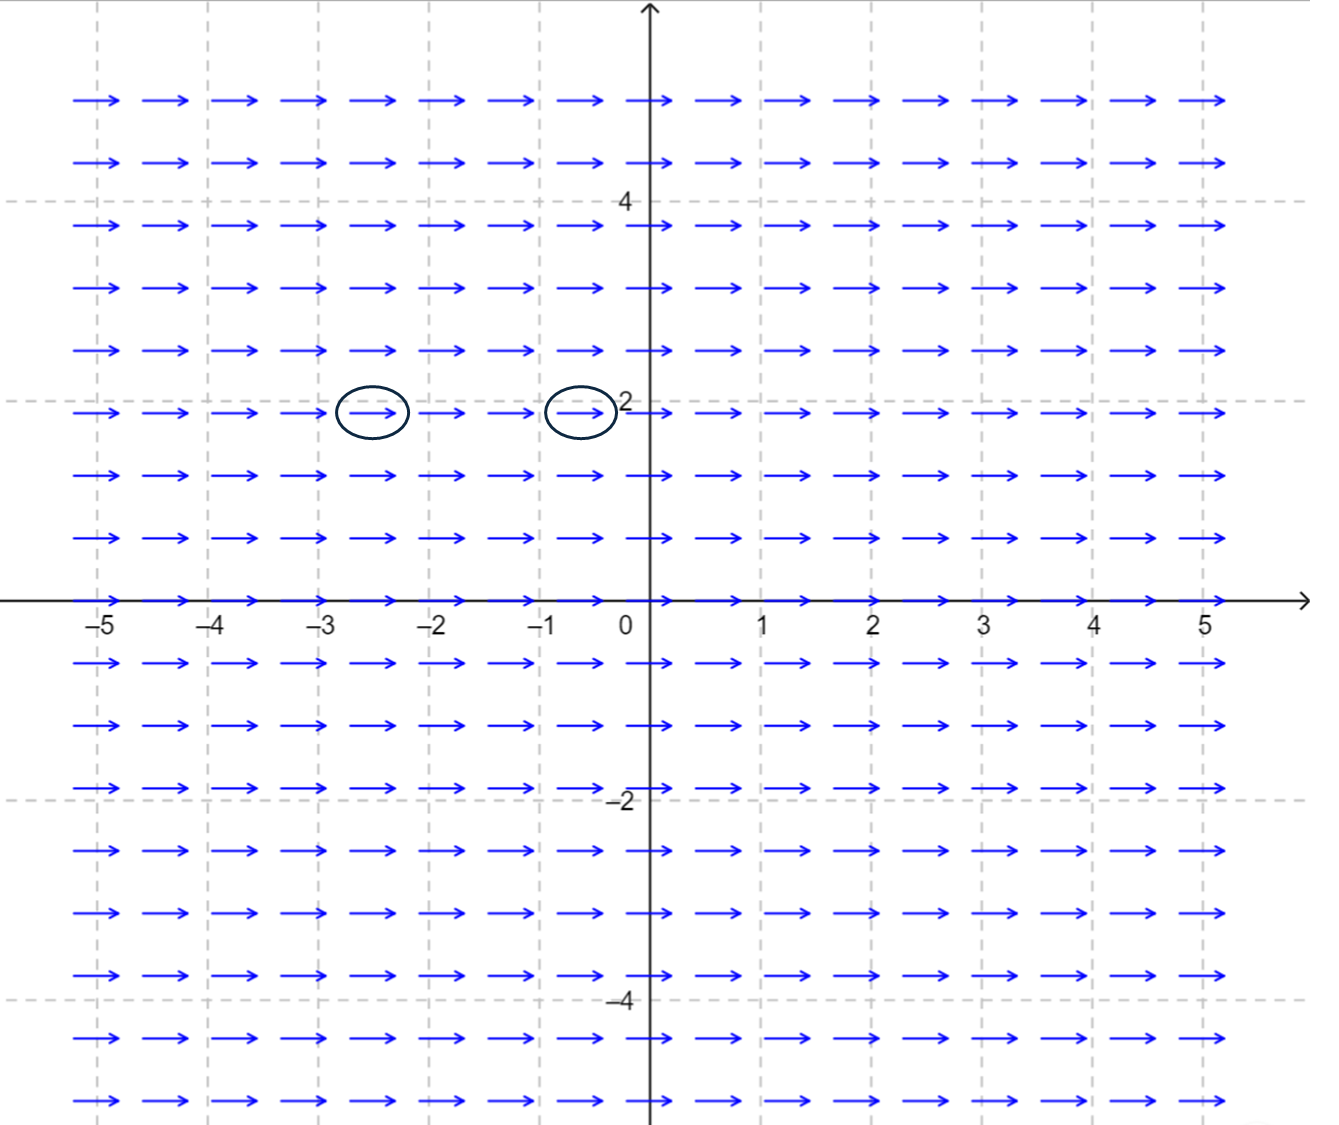
\includegraphics[width=0.9\textwidth]{images/vector_field_3.png}
            \caption{Need to compare these two vectors}
            \label{fig:sub3}
          \end{subfigure}%
          \begin{subfigure}{.5\textwidth}
            \centering   
            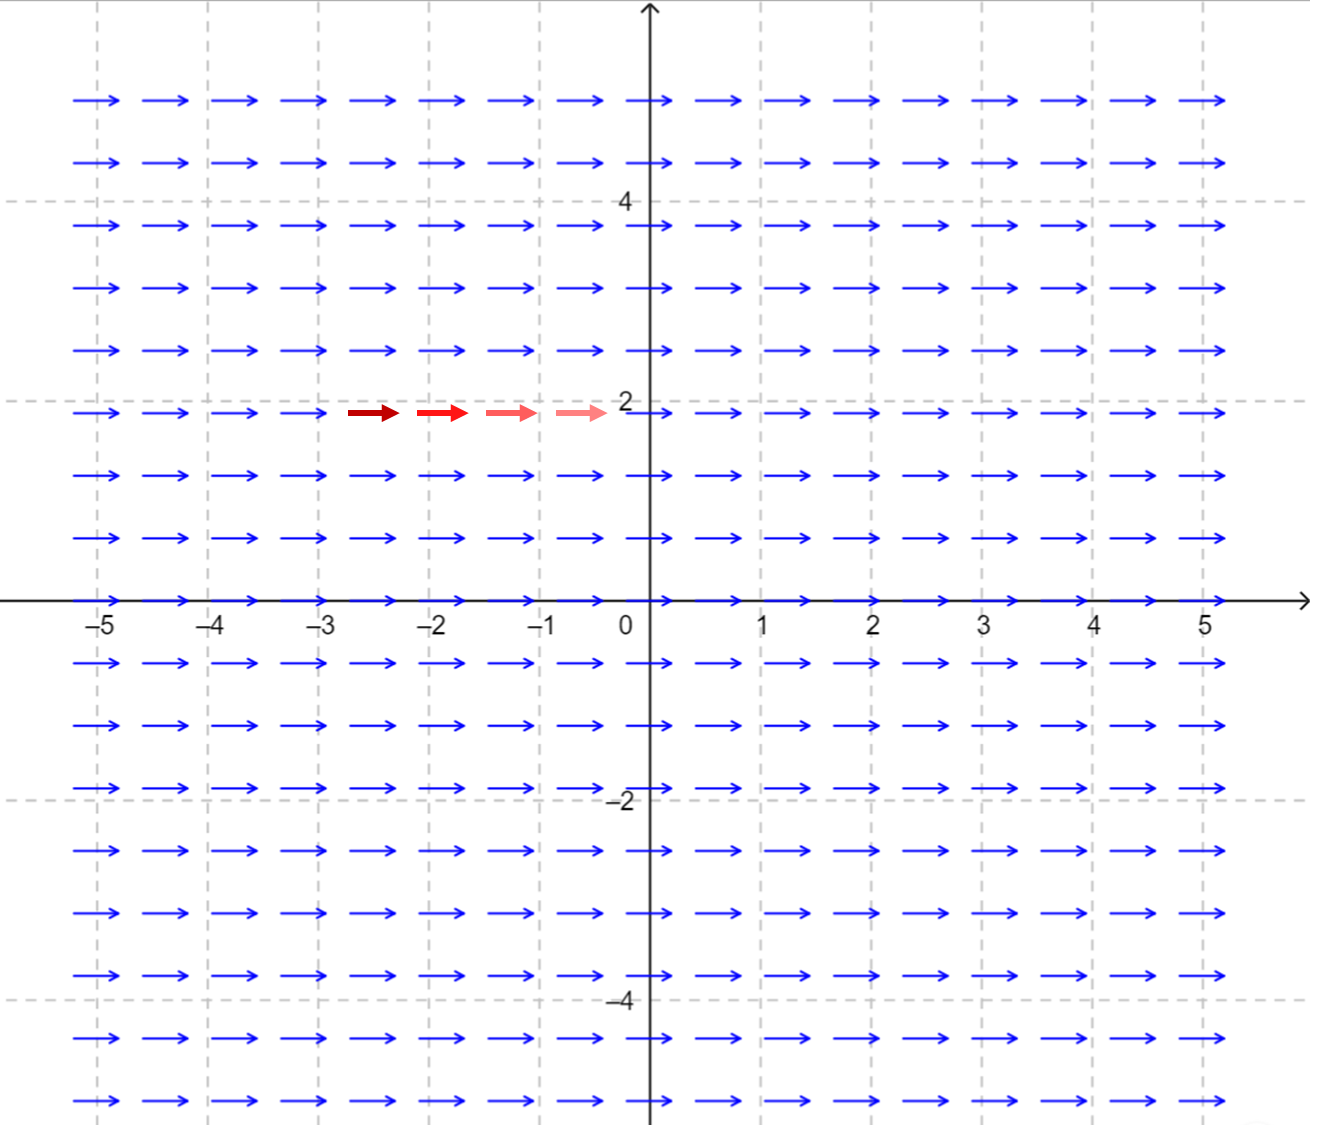
\includegraphics[width=0.9\textwidth]{images/vector_field_4.png}
            \caption{Parallel transport of a vector}
            \label{fig:sub4}
        \end{subfigure}  
    \end{figure}
    \begin{itemize}
        \item To compare two vectors on the plane we need \textbf{parallel transport}. How to generalize this on manifolds?
    \end{itemize}
\end{frame}


\subsection{Parallel transport on a sphere}
\begin{frame}{Parallel transport on a sphere (the wrong)}
\begin{figure}[h!]
    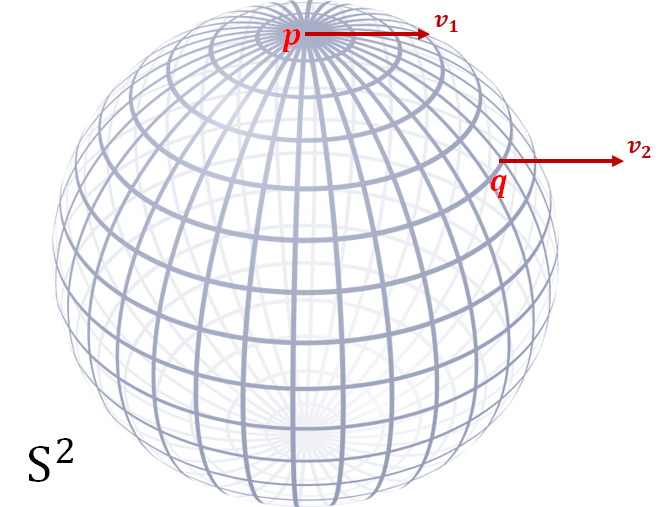
\includegraphics[width=0.5\textwidth]{images/PT_sphere_wrong.png}
\end{figure}    
\begin{itemize}
    \item While $v_1 \in \text{T}_p S^2$, clearly $v_2 \notin \text{T}_q S^2$, so we can't identify them. 
\end{itemize}
\end{frame}

\begin{frame}{Parallel transport on a sphere (the correct)}
    \begin{figure}[h!]
        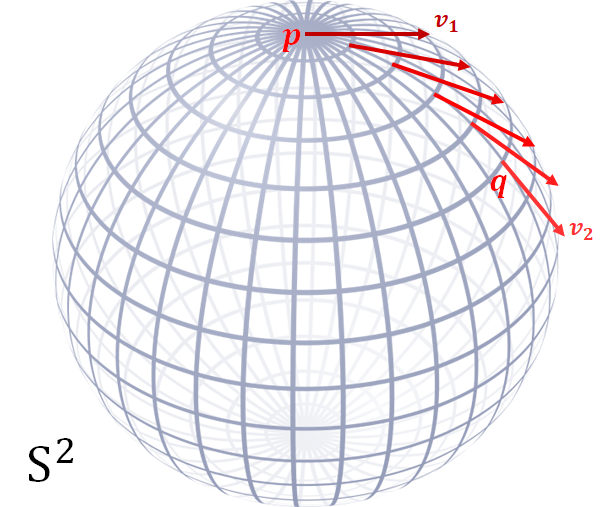
\includegraphics[width=0.5\textwidth]{images/PT_sphere_right.png}
    \end{figure}    
    \begin{itemize}
        \item Looks better, right? But there is still something to learn. 
    \end{itemize}
\end{frame}
    

\begin{frame}{Parallel transport on a sphere (the weird)}
\begin{figure}[h!]
    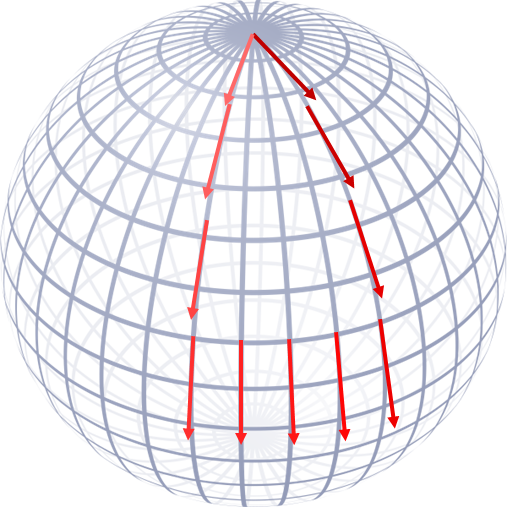
\includegraphics[width=0.4\textwidth]{images/PT_sphere.png}
\end{figure}  
\begin{itemize}
    \item We thought that we kept the vector constant, but along the loop it doesn't make sense. Then what does it mean?
\end{itemize}  
\end{frame}

\subsection{Formalization}
\begin{frame}{Formalization}
    \begin{itemize}
        \item Parallel transport keeps vectors as constant as possible.
    \end{itemize}
    \begin{figure}[h!]
        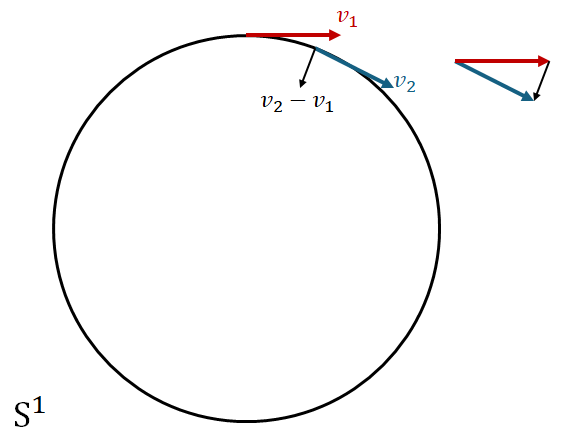
\includegraphics[width=0.4\textwidth]{images/only_normal.png}
        \caption{The change is only along the normal to the manifold}
    \end{figure}
    \begin{itemize}
        \item Given a path $c(t)$ on a manifold, a parallel transported vector field $\vec{V}(x)$ should satisfy 
        \begin{equation}
            \frac{d\vec{V}}{dt}(c(t)) = \vec{n}, \text{ or } \frac{d\vec{V}}{dt}(c(t)) - \vec{n} = 0
        \end{equation}
    \end{itemize}
\end{frame}

\subsection{Connections ignore parallel transport}
\begin{frame}{Connections ignore parallel transport} 
    \begin{itemize}
        \item Thus, when we measure change, we should substract the normal component.
        \item Equation (5.4) in the book describing a possible connection is nothing more than a very natural implementation of this idea
    \end{itemize}
    \begin{equation}
        \nabla_u V(x) = \text{Proj}_x(\text{D}_x\bar{V}[u]) 
    \end{equation}
    \begin{itemize}
        \item \textbf{Definition} If $c : I\to \mathcal{M}$ is a smooth curve and $v \in \text{T}_x \mathcal{M}$ where $x = c(0)$, then we say that a vector field $V$ along $c$ satisfying 
        \begin{equation}
            \nabla_{c^\prime(t)} V(c(t))= 0, \forall t \in I \text{ and } V(c(0)) = v
        \end{equation}
        is a {\color{blue}\textbf{parallel transport of}} $v$ along $c$. 
    \end{itemize}
\end{frame}

\begin{frame}{The formal definition of connection}
    \begin{itemize}
        \item We will mostly use the equation (5.4) as a connection, but it's possible to take something else. Well, in this case it should at least enjoy similar properties.
        \item \textbf{Definition 5.1} A {\color{blue}\textbf{connection}} on a manifold $\mathcal{M}$ is an operator 
        \begin{equation}
            \nabla : \text{T}\mathcal{M} \times \mathfrak{X}(\mathcal{M}) \to \text{T} \mathcal{M}, \quad (u, V) \mapsto \nabla_u V
        \end{equation}
        such that $\nabla_u V \in \text{T}_x \mathcal{M}$ for $u \in \text{T}_x \mathcal{M}$ and which satisfies 
        \begin{enumerate}
            \item smoothness: $(\nabla_U V)(x) : \nabla_{U(x)}V$ is a smooth vector field 
            \item linearity in $u$: $\nabla_{au+bw}V = a\nabla_u V + b \nabla_w V$
            \item linearity in $V$: $\nabla_{u}(aV+bW) = a\nabla_u V + b \nabla_u W$
            \item Leibniz' rule: $\nabla_u(fV) = \underbrace{\text{D}_x f[u]}_{\text{scalar}}  V(x) + f(x) \nabla_u V$
        \end{enumerate}
        \item \textbf{Theorem 5.2} Shows that $\nabla_u V = \text{Proj}_x(\text{D}_x\bar{V}[u])$ satisfies these properties, serving as a prototype. 
    \end{itemize}
\end{frame}


\section{Geometric motivation to algebraic operations}
\subsection{Vector fields as derivations}
\begin{frame}{Vector fields as derivations (1 / 2)}
    \begin{itemize}
        \item \textbf{Definition} A {\color{blue}\textbf{derivation}} on $\mathcal{M}$ is a linear map $\mathcal{D} : \mathfrak{F}(\mathcal{M}) \to \mathfrak{F}(\mathcal{M})$ that also satisfies the Leibniz' rule 
        \begin{equation}
            \mathcal{D}(fg) = g \mathcal{D}(f) + f \mathcal{D}(g)    
        \end{equation}
    \end{itemize}
    \begin{itemize}
        \item Typical examples on $\mathbb{R}^{n}$ are 
        \begin{equation}
            \frac{\partial}{\partial x_i}, \quad i = 1, ..., n 
        \end{equation}
        \item There is a vector field $V_i(x) = e_{x_i}$ associated with each of these examples as $V_i f(x) = D_x f[e_{x_i}]$
        \begin{figure}[h!]
            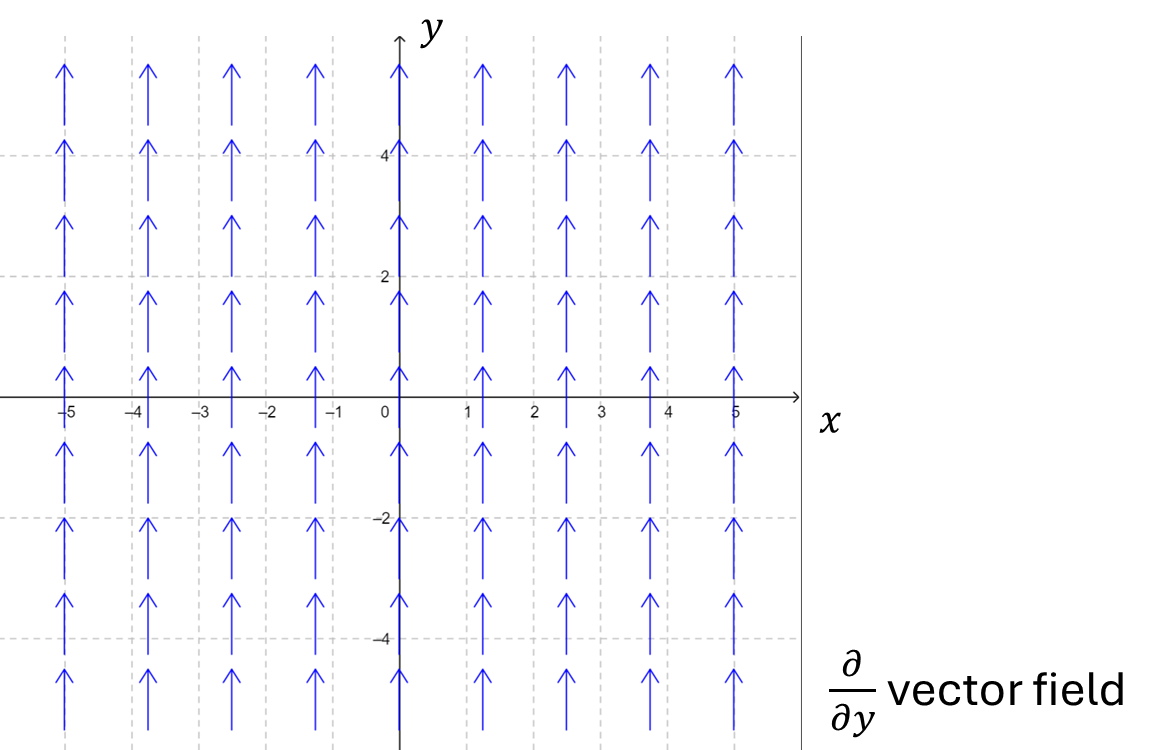
\includegraphics[width=0.4\textwidth]{images/partial_y_vector_field.png}
        \end{figure}
    \end{itemize}
    
\end{frame}
\begin{frame}{Vector fields as derivations (2 / 2)}
    \begin{itemize}
        \item Let's generalize this approach. 
        \item \textbf{Definition 5.5 (1)} Let $V \in \mathfrak{X}(\mathcal{M})$ be a vector field on a manifold $\mathcal{M}$, then for a scalar field $f \in \mathfrak{F}(\mathcal{M})$ we can get another scalar field $Vf \in \mathfrak{F}(\mathcal{M})$ as 
        \begin{equation}
            Vf(x) = \text{D}_{x}f[V(x)]
        \end{equation}
        \item This is a derivation which represents the rate of change of $f$ along the direction of $V$ at every point $x$. 
        \item This is a special case of the \textbf{Lie derivative} which represents the rate of change of a tensor field along the flow of a vector field. We will soon see another example. 
    \end{itemize}
\end{frame}

\subsection{Lie bracket motivation}
\begin{frame}{Lie bracket motivation}
    \begin{itemize}
        \item One vector field $V$ produces the flow, the other $W$ changes along it. We want to quantify this as $\mathcal{L}_V W$. 
    \end{itemize}
    \begin{figure}[h!]
        \begin{subfigure}{.5\textwidth}
            \centering  
            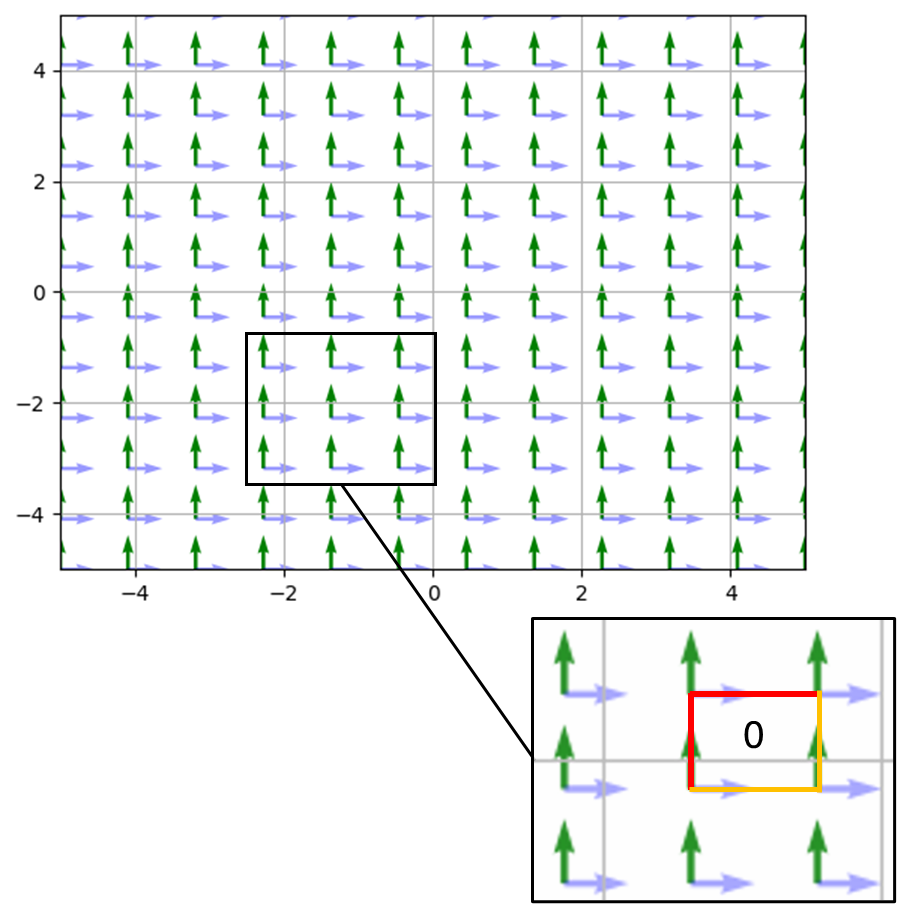
\includegraphics[width=0.8\textwidth]{images/lie_1.png}
            \caption{$V=e_2, W=e_1$}
            \label{fig:sub1}
        \end{subfigure}%
        \begin{subfigure}{.5\textwidth}
            \centering   
            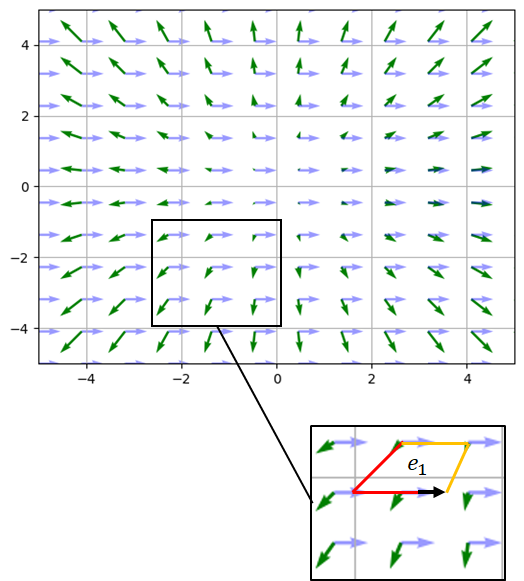
\includegraphics[width=0.75\textwidth]{images/lie_2.png}
            \caption{$V = xe_1 + ye_2, W=e_1$}
            \label{fig:sub2}
        \end{subfigure}  
    \end{figure}
\end{frame}

\subsection{Flows}
\begin{frame}{Flows (1 / 2)}
    \begin{itemize}
        \item \textbf{Definition} Let $c : I \to \mathcal{M}$ be a smooth curve, we say that $c$ is a {\color{blue}\textbf{integral curve}} of some vector field $V$ if and only if 
        \begin{equation}
            c^\prime (t) = V(c(t)), \forall t \in I
        \end{equation}
        \item Then \textbf{Definition 5.5 (1)} can alternatively be written as 
        \begin{equation}
            Vf(x) = \frac{d}{dt} (f \circ c) \Big|_{t=0} = \lim_{t \to 0 }{\frac{f(c(t)) - f(x)}{t}} = \text{D}_{x}f[V(x)]
        \end{equation}
        where $c$ is a flow s.t. $c(0) = x$. The last equality follows from \textbf{Definition 3.34} as $c^\prime(0) = V(x)$ and $c(0) = x$. 
    \end{itemize}
\end{frame}

\begin{frame}{Flows (2 / 3)}
    \begin{itemize}
        \item Suppose that for each point $p \in M$ there exists a unique integral curve of $V$ starting at $p$ and defined on $I = \mathbb{R}$. We denote it as $\theta^{(p)} : \mathbb{R} \to \mathcal{M}$. 
        \item We define a map $\theta_t : \mathcal{M} \to \mathcal{M}$ sending each $p \in M$ to the point obtained by following for time $t$ the integral curve startint at $p$
        \begin{equation}
            \theta_t(p) = \theta^{(p)}(t)
        \end{equation}
        \item Notice that $\theta_t \circ \theta_s (p) = \theta_{t+s}(p)$ and $\theta_0(p) = \theta^{(0)}(p) = p$. 
        \item Thus, we can create a map $\theta : \mathbb{R} \times \mathcal{M} \to \mathcal{M}$ which satisfies nice algebraic properties, while also having a geometric interpretation. We call it a {\color{blue}\textbf{global flow}}. 
    \end{itemize}
\end{frame}

\begin{frame}{Flows (3 / 3)}
    \begin{itemize}
        \item Let's compute the flow on a plane for $V(x, y) = xe_1 + ye_1$. Start with an integral curve 
        \begin{equation}
            \frac{dc_x}{dt} = c_x(t), \quad \frac{dc_y}{dt} = c_y(t) 
        \end{equation}
        then $c(t) = (ae^{t}, be^{t})$. 
        \item Then $\theta^{(x, y)}(t) = (xe^{t}, ye^{t})$.
    \end{itemize}
    \begin{figure}[h!]
        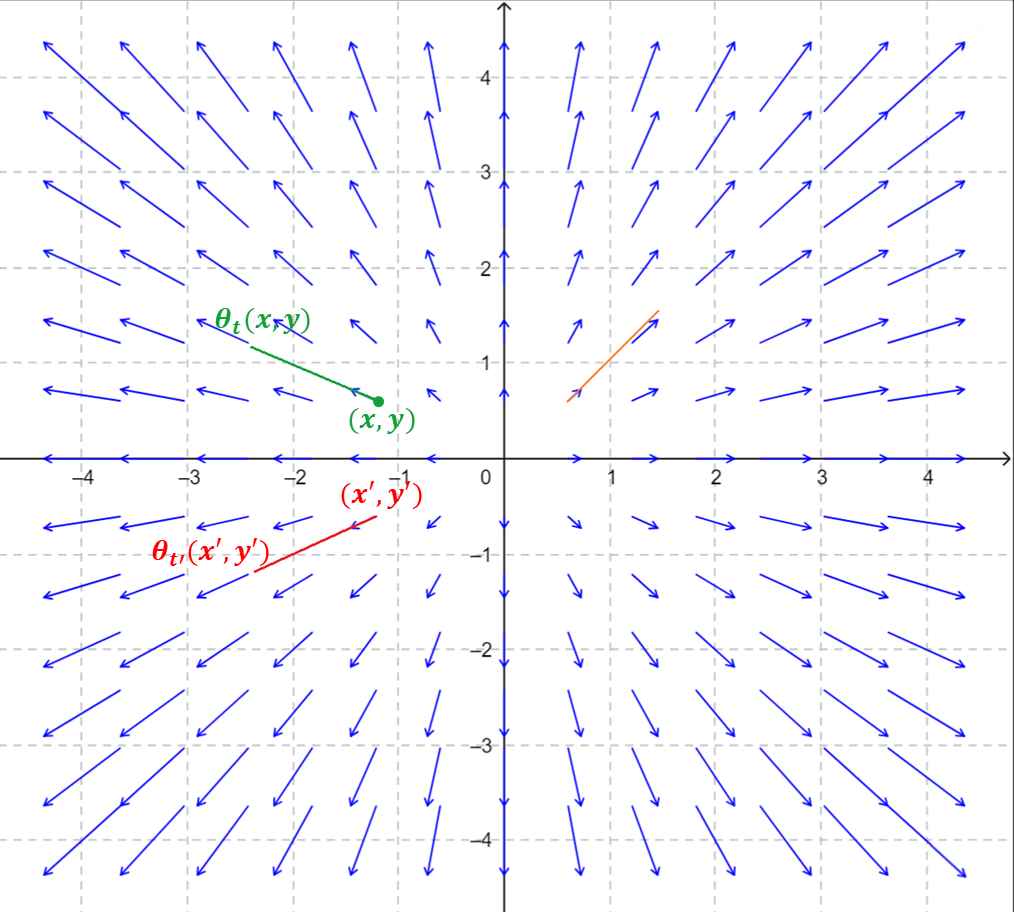
\includegraphics[width=0.4\textwidth]{images/flows.png}
    \end{figure}
\end{frame}

\subsection{Lie bracket}
\begin{frame}{Lie bracket (1 / 4)}
    \begin{itemize}
        \item Having the global flow $\theta$ associated with $V$, we can now redefine $Vf$ again as 
        \begin{equation}
            Vf(x) = \underbrace{(\mathcal{L}_V f)}_{\text{\tiny Lie derivative}}(x) := \frac{d}{dt} (f \circ \theta_t)(x) \Big|_{t = 0}
        \end{equation} 
        \item What about the Lie derivative $\mathcal{L}_V W$ of some other vector field $W$? For a fixed $t$, $\theta_t : \mathcal{M} \to \mathcal{M}$, and we can differentiate it getting $D_x\theta_t : \text{T}_{x}M \to \text{T}_{\theta_t(x)}\mathcal{M}$. Then 
        \begin{equation}
            (\mathcal{L}_V W)(x) = \frac{d}{dt} (D_x \theta_t)^{-1}[W\circ \theta_t(x)] \Big|_{t = 0}
        \end{equation}
        \item Notice how we are computing this in $\text{T}_x \mathcal{M}$.
    \end{itemize}
\end{frame}

\begin{frame}{Lie bracket (2 / 4)}
    \begin{itemize}
        \item Consider two vector fields on a plane $V(x, y) = x e_1 + ye_2$ and $W(x, y) = e_1$. We already know what $\theta_t(x, y)$ is in this case, $\theta_t(x, y) = (xe^{t}, ye^{t})$, and  
        \begin{equation}
            \text{D}_{(x, y)}\theta_t = \begin{pmatrix}
                e^{t} & 0 \\
                0 & e^{t}
            \end{pmatrix}, \quad \text{D}_{(x, y)}\theta_t = \begin{pmatrix}
                e^{-t} & 0 \\
                0 & e^{-t}
            \end{pmatrix}
        \end{equation}
        \item Notice how $(\text{D}_{(x, y)}\theta_t)^{-1} = \text{D}_{(x, y)}\theta_{-t}$, this is not a coincidence. Finally 
        \begin{equation}
            (\mathcal{L}_{V}W)(x) = \frac{d}{dt} \begin{pmatrix}
                e^{t} \\
                0
            \end{pmatrix} \Big|_{t = 0} = \begin{pmatrix}
                1 \\
                0
            \end{pmatrix} = e_1 
        \end{equation}
    \end{itemize}
\end{frame}

\begin{frame}{Lie bracket (3 / 4)}
    \begin{itemize}
        \item \textbf{Definition 5.5 (2)} Let $V, W \in \mathfrak{X}(\mathcal{M})$. A {\color{blue}\textbf{Lie bracket}} is a vector field $[V, W] = \mathcal{L}_V W$ that represents the derivative of $Y$ along the flow generated by $X$.
        \item It's possible to show that for $f \in \mathfrak{F}(\mathcal{M})$
        \begin{equation}
            \color{blue}[V, W] f = V(Wf) - W(Vf) 
        \end{equation}
        For example, in $\mathbb{R}^{n}$
        \begin{equation}
            [V_i, V_j]f = V_i(V_j f) - V_j(V_i f) = \frac{\partial}{\partial x_i} \left(\frac{\partial f}{\partial x_j}\right) - \frac{\partial}{\partial x_j} \left(\frac{\partial f}{\partial x_i}\right)  = 0
        \end{equation}
        where $V_i = e_i$. This is a result of \textbf{Clairaut's theorem}.
    \end{itemize}
\end{frame}

\begin{frame}{Lie bracket (4 / 4)}
    \begin{itemize}
        \item Returning back to our example with $V(x, y) = xe_1 + ye_2$ and $W(x, y) = e_1$ we have 
        \begin{equation}
            Wf(x,  y) = \frac{\partial f}{\partial x}, \quad Vf(x, y) = x \frac{\partial f}{\partial x} + y \frac{\partial f}{\partial y}
        \end{equation}
        and 
        \begin{align}
            V(Wf)(x, y) &= x \frac{\partial^2 f}{\partial x^2} + y \frac{\partial^2 f}{\partial y \partial x} \\
            W(Vf)(x, y) &= \frac{\partial f}{\partial x} + x \frac{\partial^2 f}{\partial x^2} + y \frac{\partial^2 f}{\partial x \partial y}
        \end{align}
        so 
        \begin{equation}
            [V, W]f = \frac{\partial f}{\partial x}
        \end{equation}
        \item This is precisely the action of $\mathcal{L}_V W = e_1$ we computed previously on $f$. 
    \end{itemize}
\end{frame}

\subsection{Torsion}
\begin{frame}{Torsion}
    \begin{itemize}
        \item Two vector fields $u$ and $v$. 
        \item Compute $\nabla_v u$ and $\nabla_u v$ using parallel transport
        \item Compute the Lie bracket $[u, v]$
        \item Closure failure $T(u, v) = \nabla_u v - \nabla_v u - [u, v]$ is known as {\color{blue}\textbf{torsion}}
    \end{itemize}
    \begin{figure}[h!]
        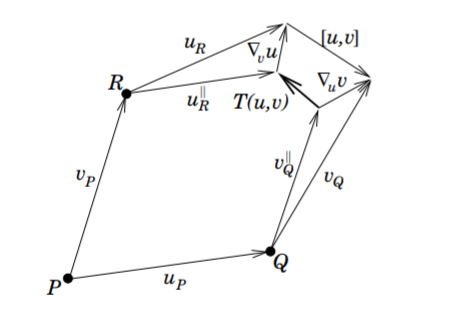
\includegraphics[width=0.5\textwidth]{images/torsion.png}
    \end{figure}
\end{frame}

\subsection{The canonical Euclidean connection}
\begin{frame}{The canonical Euclidean connection}
    \begin{itemize}
        \item \textbf{Definition} Let $U, V, W\in \mathfrak{X}(\mathcal{M})$. A connection $\nabla$ is called 
        \begin{enumerate}
            \item {\color{blue}\textbf{Torsion-free}} or {\color{blue}\textbf{symmetric}} if and only if 
            \begin{equation}
                T(V, W) = \nabla_V W - \nabla_W V - [V, W] = 0 
            \end{equation}
            \item {\color{blue}\textbf{Compatible with the metric}}
            \begin{equation}
                U\langle V, W\rangle = \langle \nabla_U V, W\rangle + \langle V, \nabla_U W \rangle 
            \end{equation}
            this one implies that the metric is constant w.r.t. $\nabla$, i.e. $\nabla_U \langle \cdot, \cdot\rangle = 0$. 
        \end{enumerate}
        \item \textbf{Theorem 5.7} The Riemannian connection on a Euclidean space $\mathcal{E}$ with any Euclidean metric $\langle \cdot, \cdot \rangle$ is $\nabla_u V = \text{D}_x V[u]$: the {\color{blue}canonical Euclidean connection}. 
    \end{itemize}
\end{frame}

\begin{frame}{Proof of Theorem 5.7}
    \begin{itemize}[<+->]
        \item Take $U, V, W \in \mathfrak{X}(\mathcal{M})$. We start by showing compatability with the metric, that is 
        \begin{equation}
            U\langle V, W\rangle = \langle \nabla_U V, W\rangle +\langle V, \nabla_U W\rangle
        \end{equation}
        \item Taylor: 
        \begin{align*}
            V(x+tU(x)) &= V(x) + t \text{D}V(x)[U(x)] + O(t^2) = \\
            &= V(x) + t(\nabla_U V)(x) + O(t^2 )
        \end{align*}
        \item We can do the same thing for $W$. 
    \end{itemize}
\end{frame}

\begin{frame}{Proof of Theorem 5.7}
    \begin{itemize}[<+->]
        \item Take a scalar field $f = \langle U, W\rangle$ 
        \item Then 
        \begin{align*}
            (Uf)(x) &:= D_xf[U(x)] = \\
            &= \lim_{t\to 0}{\frac{\langle V(x+tU(x)), W(t+tU(x)) \rangle - \langle  V(x), W(x)\rangle }{t}} 
        \end{align*}
    \end{itemize}
\end{frame}

\begin{frame}{Proof of Theorem 5.7}
    \begin{itemize}
        \item Take a scalar field $f = \langle U, W\rangle$ 
        \item Then 
        \begin{align*}
            &(Uf)(x) := D_xf[U(x)] = \\
            &= \lim_{t\to 0}{\frac{\langle {\color{orange}V(x+tU(x))}, {\color{blue}W(t+tU(x))} \rangle - \langle  V(x), W(x)\rangle }{t}} = \\
            &= \lim_{t\to 0}{\frac{\langle {\color{orange}V(x) + t(\nabla_U V)(x)}, {\color{blue}W(x) + t(\nabla_U W)(x) }\rangle - \langle V(x), W(x)\rangle }{t}} = \\
            &= \left(\langle \nabla_U V, W\rangle +\langle  V, \nabla_U W\rangle\right)(x)
        \end{align*}
    \end{itemize}
\end{frame}

\begin{frame}{Proof of Theorem 5.7}
    \begin{itemize}[<+->]
        \item Now, let's prove that it's symmetric. First, notice that 
        \begin{equation}
            (Vf)(x) = \text{D}f(x)[V(x)] = \langle \text{grad}f(x), V(x)\rangle_x 
        \end{equation}
        \item $\text{grad} f(x)$ is a vector field, so 
        \begin{equation}
            U(Vf)  = U\langle \text{grad}f, V\rangle = \langle \nabla_U (\text{grad} f), V\rangle + \langle \text{grad} f, \nabla_U V\rangle 
        \end{equation}
        \item But $\nabla_U (\text{grad} f) = \text{Hess}f[U]$ is a vector field s.t. 
        \begin{equation}
            (\text{Hess}f[U])(x) = \text{Hess}f(x)[U(x)] = \nabla_{U(x)}(\text{grad} f) 
        \end{equation}
        \item Thus 
        \begin{equation}
            U(Vf) = \langle \text{Hess}f[U], V\rangle + \langle \text{grad}f, \nabla_U V\rangle
        \end{equation}
    \end{itemize}
\end{frame}

\begin{frame}{Proof of Theorem 5.7}
    \begin{itemize}[<+->]
        \item We have for $f \in \mathfrak{F}(\mathcal{M})$
        \begin{align*}
            U(Vf) &= \langle \text{Hess}f[U], V\rangle + \langle \text{grad}f, \nabla_U V\rangle \\
            V(Uf) &= \langle \text{Hess}f[V], U\rangle + \langle \text{grad}f, \nabla_V U\rangle
        \end{align*}
        \item But $\text{Hess} f$ is self-adjoint (Clairaut's theorem), so
        \begin{equation}
            \langle \text{Hess}f[U], V\rangle = \langle \text{Hess}f[V], U\rangle
        \end{equation}
        \item Thus 
        \begin{equation}
            [U, V]f = \langle \text{grad} f, \nabla_U V - \nabla_V U\rangle = (\nabla_U V - \nabla_V U)f 
        \end{equation}
        and so 
        \begin{equation}
            [U, V] = \nabla_U V - \nabla_V U 
        \end{equation}
    \end{itemize}
\end{frame}

\subsection{Symmetricity of connection (5.4)}
\begin{frame}{Symmetricity of connection (5.4)}
    \begin{itemize}
        \item \textbf{Theorem 5.8} Let $\mathcal{M}$ be an embedded submanifold of a Euclidean space $\mathcal{E}$. The connection $\nabla$ defined by 
        \begin{equation}
            \nabla_u V = \text{Proj}_x (\text{D}_x\bar{V}[u])
        \end{equation}
        is symmetric. 
    \end{itemize}
\end{frame}

\begin{frame}{Proof of Theorem 5.8}
    \begin{itemize}[<+->]
        \item Let $\bar{\nabla}$ denote the canonical Euclidean connection on $\mathcal{E}$. 
        \item If $\mathcal{M}$ is open, then $\nabla = \bar{\nabla} |_\mathcal{M}$ and there is nothing to prove. 
        \item Let $O$ be a neighborhood of $\mathcal{M}$ in $\mathcal{E}$.
        \item Consider $U, V \in \mathfrak{X}(\mathcal{M})$ and $f \in \mathfrak{F}(\mathcal{M})$ with smooth extensions $\bar{U}, \overline{V} \in \bar{X}(O)$ and $\bar{f} \in \mathfrak{F}(O)$. 
        \item Then 
        \begin{align*}
            [U, V]f &= U(Vf) - V(Uf) = U(\bar{V}\bar{f}|_f) - V((\bar{U} \bar{f} |_\mathcal{M})) = \\
            &= (\bar{U}(\bar{V} \bar{f}))|_\mathcal{M} - (\bar{V}(\bar{U}\bar{f}))|_\mathcal{M} = ([\bar{U}, \bar{V}]\bar{f})|_\mathcal{M} = \\
            &= (\underbrace{(\bar{\nabla}_{\bar{U}} \bar{V} - \bar{\nabla}_{\bar{V} } \bar{U})}_{\bar{W}} \bar{f})_\mathcal{M} = (\bar{W} \bar{f})|_\mathcal{M}
        \end{align*}
    \end{itemize}
\end{frame}

\begin{frame}{Proof of Theorem 5.8}
    \begin{itemize}[<+->]
        \item We need to show that $\bar{W}(x) \in \text{T}_x \mathcal{M}$ for all $x$
        \item Let $\bar{h} : O' \to \mathbb{R}^{k}$ be a local defining function for $\mathcal{M}$ around $x$, i.e. $\mathcal{M} \cap O' = \bar{h}^{-1}(0)$ and we can also ensure $O' \subseteq O$. 
        \item Consider $h = \bar{h}|_{\mathcal{M} \cap O'} = 0$, then 
        \begin{equation}
            0 = [U, V]h = (\bar{W} \bar{h})|_{\mathcal{M} \cap O'}
        \end{equation}
        \item So at $x$ 
        \begin{equation}
            0 = (\bar{W}\bar{h})(x) \overset{\Delta}{=} \text{D}\bar{h}(x) [\bar{W}(x)]
        \end{equation}
        \item Thus $\bar{W}(x) \in \text{ker} \text{D}\bar{h}(x)$ which is equivalent to $\bar{W}(x) \in \text{T}_x \mathcal{M}$
    \end{itemize}
\end{frame}

\begin{frame}{Proof of Theorem 5.8}
    \begin{itemize}
        \item Finally, we can write 
        \begin{equation*}
            W = \bar{W}|_\mathcal{M} = \text{Proj}(\bar{W}) = \text{Proj}(\bar{\nabla}_{\bar{U}} \bar{V} - \bar{\nabla}_{\bar{V}} \bar{U}) \overset{\Delta}{=} \nabla_U V - \nabla_V U
        \end{equation*}
        \item But then 
        \begin{equation}
            [U, V]f = (\bar{W}\bar{f})|_\mathcal{M} = Wf = (\nabla_U V - \nabla_V U)f
        \end{equation}
    \end{itemize}
\end{frame}

\end{document}